\documentclass[11pt]{article}
\usepackage[a4paper,margin=1in]{geometry}
\usepackage{amsmath,amssymb,amsthm,mathtools}
\usepackage{booktabs}
\usepackage{enumitem}
\usepackage{float}
\usepackage{graphicx}
\usepackage{hyperref}
\usepackage[nameinlink,capitalise]{cleveref}
\usepackage[numbers,sort&compress]{natbib}

\newtheorem{theorem}{Theorem}[section]
\newtheorem{proposition}[theorem]{Proposition}
\newtheorem{corollary}[theorem]{Corollary}
\theoremstyle{remark}
\newtheorem{remark}[theorem]{Remark}

\newcommand{\norm}[1]{\left\lVert#1\right\rVert}
\newcommand{\HS}{\mathfrak S_2}
\newcommand{\cE}{\mathcal E}
\newcommand{\tr}{\operatorname{tr}}
\newcommand{\spr}{\operatorname{spr}}
\newcommand{\diag}{\operatorname{diag}}

\title{Flag-Adapted Schur--Stein Metrics for Directional Hardy Packets\\
\large Exact Dissipation and the Outer-Packet Bottleneck}
\author{Liang Wang}
\date{July 2026}

\begin{document}
\maketitle

\begin{abstract}
The directional small-noise program has reduced its remaining analytic gate
to two Hilbert--Schmidt Hardy energies.  RH-58 replaced oblique radial Riesz
blocks by unitary Schur packets, but a scalar sum over all upper-triangular
paths grew much faster than the exact energies.  This paper retains the
Schur flag and replaces that path ledger by positive anisotropic metrics.

For every stable finite upper-triangular block matrix, we solve a canonical
Lyapunov equation on each diagonal block and prove that hierarchical positive
scalings produce a block diagonal metric $P$ with
$R=P-T^*PT\succ0$.  This gives an exact flag-compatible stability theorem.
For an observation $Y$, the constant
$\kappa=\norm{YR^{-1/2}}_2^2$ makes $\kappa P$ a positive Stein
supersolution.  Applying a separate prefix metric to each initial Schur
packet bounds every diagonal entry of the RH-58 packet Gram.  The complete
dissipation $R$ is always at least as sharp as the usual one-number
contraction estimate.  A two-scalar-block formula also proves an endpoint
tradeoff: when an outer packet is seen through a nonzero inner observation,
the metric cost diverges at both boundaries of the admissible scaling
interval.

The five-scale all-column binary64 audit gives a substantial but incomplete
gain.  At $\sigma=0.01$, the left/right packetwise metric uppers are $19.2196$
and $12.1382$, compared with the RH-58 absolute-path uppers $1922.40$ and
$380.40$ and exact energies $1.4681$ and $1.7603$.  The remaining loss is
concentrated in the outer packet, whose metric uppers are $13.7336$ and
$6.7965$.  The fitted total growth exponents are still $0.898$ and $0.763$;
therefore no dyadically uniform or polylogarithmic Stage A1 estimate follows.
A 256-bit Arb calculation certifies the formulas on one two-scalar-block
model only.  No arithmetic trace formula, self-adjoint realization, or
Hilbert--Polya conclusion is claimed.
\end{abstract}

\noindent\textbf{Keywords:} Schur flag; Stein inequality; Lyapunov metric;
Hardy energy; block diagonal stability; nonnormal operator; small noise.

\medskip
\noindent\textbf{MSC 2020:} 47A10; 47B65; 93B07; 93D05; 65F35.

\section{Introduction}

RH-48--RH-50 reduced small-noise intrinsic Riesz identification to two
directional Hardy energies of residue-deflated bulk operators
\citep{WangIntrinsic2026,WangDirectional2026,WangHardy2026}.  The exact
finite-dimensional energy is benign on every stored scale, but a proof must
remain quantitative as the noise decreases.  RH-56 ruled out a uniform
strong-space route \citep{WangHardyBarrier2026}; RH-57 showed that fixed
radial Riesz blocks become severely oblique
\citep{WangRieszOverlap2026}.

RH-58 then moved to a unitary Schur basis and proved two exact positive packet
Gram identities \citep{WangSchurGram2026}.  That coordinate change removed
the projector wall: the measured input and output packet budgets stayed near
the exact Hardy energies.  However, bounding every feed-forward Schur path
independently produced smallest-scale uppers $1922.40$ and $380.40$.  The
path argument had discarded the Hilbert-space geometry that motivated the
Schur basis.

The natural repair is a positive anisotropic metric.  This idea has two
logically separate parts.
\begin{enumerate}[leftmargin=2.2em]
 \item Does every stable Schur flag admit a compatible block diagonal
       Lyapunov metric?
 \item Can such metrics control the directional packet energies with a
       noise-uniform quantitative budget?
\end{enumerate}
The answer to the first question is yes.  We give an explicit construction
from local Lyapunov equations and diagonal block scalings.  The second answer
is mixed.  Exact dissipation removes most of the RH-58 path proliferation,
but the outer packet develops a strong endpoint cost on the two finest
levels.  Thus RH-59 identifies a much narrower obstruction without closing
Stage A1.

\subsection*{Contributions and boundary}

\begin{enumerate}[leftmargin=2.2em]
 \item We prove flag-compatible block diagonal stability for every finite
       stable Schur partition.
 \item We convert the complete metric dissipation into a positive
       packetwise observability Stein supersolution.
 \item We prove that exact dissipation dominates both the global contraction
       estimate and its scalar block-norm comparison.
 \item We derive a two-block endpoint tradeoff and audit the resulting
       packet certificates on five all-column folded-Gaussian levels.
\end{enumerate}

The matrix theorems are exact finite-dimensional statements.  The production
Schur forms, optimized scalings, fitted powers, and dense Lyapunov solves are
binary64 diagnostics.  No continuum regularity of the noise-dependent Schur
flags or uniform control of their hierarchical weights is proved.

\section{Directional Hardy packets}
\label{sec:setup}

Let $A$ be a stable finite matrix, $X$ an input matrix, and $Y$ an
observation matrix.  The Hardy energy is
\begin{equation}
 \cE^2=\sum_{m\ge0}\norm{YA^mX}_{\HS}^2
 =\tr(X^*OX),
 \qquad O-A^*OA=Y^*Y.
 \label{eq:hardy}
\end{equation}
The two RH-50 directions have this form after the radius rescaling
$A=r^{-1}N$, with $r=0.85$ in the audit.

Choose a unitary Schur partition
\citep{GolubVanLoan2013,HornJohnson2013}
\begin{equation}
 A=QTQ^*,\qquad
 T=\begin{pmatrix}
 D_1&T_{12}&\cdots&T_{1J}\\
 0&D_2&\cdots&T_{2J}\\
 \vdots&\ddots&\ddots&\vdots\\
 0&\cdots&0&D_J
 \end{pmatrix}.
 \label{eq:schur}
\end{equation}
Write $\widehat X=Q^*X$, $\widehat Y=YQ$, and let $E_j$ be the orthogonal
coordinate projections.  The input packets are $X_j=E_j\widehat X$.  Their
complete responses
\begin{equation}
 F_j=(\widehat YT^mX_j)_{m\ge0}
 \label{eq:packet-response}
\end{equation}
have Gram matrix $K_{ij}=\langle F_i,F_j\rangle$.  In particular,
\begin{equation}
 e_j^2:=K_{jj}=\tr(X_j^*\widehat OX_j),
 \qquad \widehat O=Q^*OQ.
 \label{eq:packet-energy}
\end{equation}
RH-58 proved
\begin{equation}
 \cE\le\sum_{j=1}^Je_j,
 \qquad
 \cE^2\le\theta\sum_{j=1}^Je_j^2,
 \label{eq:packet-synthesis}
\end{equation}
where $\theta$ is the largest eigenvalue of the normalized packet Gram.
The present task is to bound the diagonal packet energies without summing
every triangular path absolutely.

Upper triangularity supplies the key localization.  The prefix
\begin{equation}
 \mathcal H^{(j)}=E_1\mathcal H\oplus\cdots\oplus E_j\mathcal H
 \label{eq:prefix}
\end{equation}
is invariant under $T$, and the orbit of $X_j$ remains inside this prefix.
We may therefore choose a different positive metric for each packet.

\section{Canonical flag metrics}
\label{sec:flag}

For every diagonal block, let $H_i$ be the local Lyapunov metric
\citep{LancasterRodman1995,ZhouDoyleGlover1996}
\begin{equation}
 H_i-D_i^*H_iD_i=I,
 \qquad
 H_i=\sum_{m\ge0}(D_i^*)^mD_i^m\succ0.
 \label{eq:local-metric}
\end{equation}
Define normalized couplings and their scalar comparison by
\begin{equation}
 B_{ij}=H_i^{1/2}T_{ij}H_j^{-1/2},
 \qquad c_{ij}=\norm{B_{ij}}_2
 \quad(i\le j).
 \label{eq:normalized-blocks}
\end{equation}
The matrix $C=(c_{ij})$ is upper triangular.

\begin{theorem}[Flag-compatible block metric]
\label{thm:flag-metric}
Let $T$ be a finite stable upper-triangular block matrix.  For positive
numbers $s_1,\ldots,s_J$, put
\begin{equation}
 P_s=\bigoplus_{i=1}^Js_i^2H_i,
 \qquad S_s=P_s^{1/2}TP_s^{-1/2}.
 \label{eq:scaled-metric}
\end{equation}
Then
\begin{equation}
 \norm{S_s}_2
 \le
 \norm{\diag(s_i)C\diag(s_i)^{-1}}_2.
 \label{eq:comparison}
\end{equation}
Moreover,
\begin{equation}
 c_{ii}^2=1-\frac{1}{\lambda_{\max}(H_i)}<1.
 \label{eq:local-contraction}
\end{equation}
Consequently there exist positive scales $s_i$ for which
\begin{equation}
 P_s-T^*P_sT\succ0.
 \label{eq:flag-dissipation}
\end{equation}
The same assertion holds on every invariant prefix.
\end{theorem}

\begin{proof}
For a block vector $v=(v_j)$, put $u_j=\norm{v_j}$.  The $i$th block of
$S_sv$ is bounded by
\[
 \sum_{j\ge i}\frac{s_i}{s_j}c_{ij}u_j.
\]
Taking the Euclidean norm over $i$ proves \eqref{eq:comparison}.  From
\eqref{eq:local-metric},
\[
 B_{ii}^*B_{ii}
 =I-H_i^{-1},
\]
which gives \eqref{eq:local-contraction}.

Choose $0<\varepsilon<1$ and $s_i=\varepsilon^{J-i}$.  Every strictly
upper entry of the scaled comparison is multiplied by
$\varepsilon^{j-i}$, while its diagonal is fixed.  As
$\varepsilon\downarrow0$, its spectral norm tends to
$\max_i c_{ii}<1$.  Hence \eqref{eq:comparison} is strictly below one for
all sufficiently small $\varepsilon$.  Finally,
\[
 P_s-T^*P_sT
 =P_s^{1/2}(I-S_s^*S_s)P_s^{1/2}\succ0.
\]
Restricting the construction to the first $j$ blocks proves the prefix
statement.
\end{proof}

\begin{remark}[Existence is not a uniform estimate]
The proof may require $s_1\ll s_2\ll\cdots\ll s_J$.  Such a hierarchy can
make an inner observation expensive in the dual metric.  The theorem solves
finite-dimensional compatibility, not the small-noise endpoint budget.
\end{remark}

\section{Exact-dissipation Stein supersolutions}
\label{sec:supersolution}

Fix packet $j$ and work on its invariant prefix.  Let $P_s$ be any metric
from \cref{thm:flag-metric} with
\begin{equation}
 R_s=P_s-(T^{(j)})^*P_sT^{(j)}\succ0.
 \label{eq:dissipation}
\end{equation}
Write $Y^{(j)}$ for the observation restricted to this prefix and define
\begin{equation}
 \kappa_{s,j}=\norm{Y^{(j)}R_s^{-1/2}}_2^2.
 \label{eq:kappa}
\end{equation}

\begin{theorem}[Packetwise exact-dissipation certificate]
\label{thm:packet-certificate}
The matrix $\widetilde O_{s,j}=\kappa_{s,j}P_s$ satisfies
\begin{equation}
 \widetilde O_{s,j}-(T^{(j)})^*\widetilde O_{s,j}T^{(j)}
 \succeq (Y^{(j)})^*Y^{(j)}.
 \label{eq:stein-super}
\end{equation}
Therefore the exact packet energy obeys
\begin{equation}
 \boxed{
 e_j^2\le u_{s,j}^2
 :=\kappa_{s,j}s_j^2\norm{H_j^{1/2}X_j}_{\HS}^2.}
 \label{eq:packet-upper}
\end{equation}
Consequently
\begin{equation}
 \cE\le\sum_{j=1}^Ju_{s^{(j)},j}
 \label{eq:absolute-synthesis}
\end{equation}
for arbitrary feasible packet-specific metrics.  If an independent packet
coherence bound $\theta$ is available, then also
\begin{equation}
 \cE^2\le\theta\sum_{j=1}^Ju_{s^{(j)},j}^2.
 \label{eq:coherent-synthesis}
\end{equation}
\end{theorem}

\begin{proof}
By the definition of operator norm,
\[
 (Y^{(j)})^*Y^{(j)}\preceq\kappa_{s,j}R_s,
\]
which is exactly \eqref{eq:stein-super}.  Iterating the positive Stein
residual and using stability gives
$O^{(j)}\preceq\widetilde O_{s,j}$.  Testing this inequality on $X_j$
proves \eqref{eq:packet-upper}.  The triangle inequality for the complete
packet responses gives \eqref{eq:absolute-synthesis}; substituting
$e_j\le u_{s^{(j)},j}$ into \eqref{eq:packet-synthesis} gives
\eqref{eq:coherent-synthesis}.
\end{proof}

The complete dissipation is sharper than reducing the metric to one
contraction number.

\begin{proposition}[Dissipation versus contraction]
\label{prop:dominance}
Let $q_s=\norm{P_s^{1/2}T^{(j)}P_s^{-1/2}}_2<1$.  Then
\begin{equation}
 \kappa_{s,j}
 \le\frac{\norm{Y^{(j)}P_s^{-1/2}}_2^2}{1-q_s^2},
 \label{eq:contraction-kappa}
\end{equation}
and $q_s$ is bounded by the scalar comparison in
\eqref{eq:comparison}.
\end{proposition}

\begin{proof}
The factorization in \cref{thm:flag-metric} gives
$R_s\succeq(1-q_s^2)P_s$.  Inverting reverses the Loewner order and proves
\eqref{eq:contraction-kappa}.  The final statement is
\eqref{eq:comparison}.
\end{proof}

This distinction matters numerically.  At many optimized production
weights, the exact normalized matrix is contractive even though the scalar
block-norm comparison exceeds one.

\section{A two-block endpoint tradeoff}
\label{sec:tradeoff}

The remaining metric loss is not only an optimization artifact.  It already
appears in the real two-scalar-block model
\begin{equation}
 T=\begin{pmatrix}a&\gamma\\0&b\end{pmatrix},
 \qquad P=\diag(p_1,p_2),
 \qquad Y=(y_1,y_2),
 \label{eq:two-block}
\end{equation}
where $|a|,|b|<1$ and $\gamma\ne0$.

\begin{proposition}[Endpoint coercivity]
\label{prop:two-block}
Put $\alpha=1-a^2$, $\delta=1-b^2$, and normalize $p_2=1$,
$t=p_1/p_2$.  Then $R=P-T^*PT$ is positive definite exactly when
\begin{equation}
 0<t<\frac{\alpha\delta}{\gamma^2}.
 \label{eq:two-block-interval}
\end{equation}
On this interval the sharp Stein multiplier is
\begin{equation}
 \kappa(t)
 =\frac{
 y_1^2(\delta-\gamma^2t)
 +2a\gamma y_1y_2t
 +\alpha y_2^2t}
 {t(\alpha\delta-\gamma^2t)}.
 \label{eq:two-block-kappa}
\end{equation}
If $y_1\ne0$ and $a\gamma y_1+\alpha y_2\ne0$, then
\begin{equation}
 \kappa(t)\longrightarrow+\infty
 \quad\text{at both endpoints of \eqref{eq:two-block-interval}}.
 \label{eq:endpoint-blowup}
\end{equation}
Hence an outer source packet has a finite interior optimal scaling, but no
extreme hierarchy removes its inner-observation cost.
\end{proposition}

\begin{proof}
Direct multiplication gives
\[
 R=\begin{pmatrix}
 \alpha t&-a\gamma t\\
 -a\gamma t&\delta-\gamma^2t
 \end{pmatrix},
 \qquad
 \det R=t(\alpha\delta-\gamma^2t).
\]
Sylvester's criterion proves \eqref{eq:two-block-interval}.  Since $Y$ has
one row, $\kappa=YR^{-1}Y^*$, which gives
\eqref{eq:two-block-kappa}.  The lower-end divergence follows from
$y_1\ne0$.  At the upper endpoint the numerator vanishes only in the
excluded alignment $a\gamma y_1+\alpha y_2=0$.  This proves
\eqref{eq:endpoint-blowup}.
\end{proof}

\section{Five-scale deterministic audit}
\label{sec:audit}

\subsection{Construction}

We use exactly the RH-58 all-column folded-Gaussian family
\[
 (\sigma,N)=(0.16,32),(0.08,64),(0.04,128),(0.02,256),(0.01,512),
 \qquad N\sigma=5.12,
\]
the Hardy radius $r=0.85$, and physical radial cuts
\begin{equation}
 0.15,\qquad0.35,\qquad0.55.
 \label{eq:cuts}
\end{equation}
Empty Schur bands are omitted.  For every active diagonal block we solve
\eqref{eq:local-metric} densely.  For packet $j$ we fix $s_j=1$, first find
a feasible seed from the scalar comparison, and then minimize the exact
binary64 value in \eqref{eq:packet-upper} over the remaining logarithmic
scales.  The optimizer only proposes weights.  Acceptance requires direct
positive dissipation with minimum eigenvalue above $10^{-8}$ and a checked
Stein supersolution residual.

The exact observability Gramian is solved independently and supplies the
packet diagonals used for comparison.  Every optimizer terminated
successfully.  None of these floating-point checks is an interval proof.

\subsection{Route comparison}

\begin{table}[H]
\centering
\small
\begin{tabular}{@{}r|rr|rr|rr@{}}
\toprule
&\multicolumn{2}{c|}{exact $\cE$}
&\multicolumn{2}{c|}{RH-59 metric upper}
&\multicolumn{2}{c}{RH-58 path upper}\\
$\sigma$&left&right&left&right&left&right\\
\midrule
0.16&0.9040&1.0026&1.1719&1.5183&1.59&1.78\\
0.08&1.1626&1.2653&2.1206&2.4307&4.41&4.15\\
0.04&1.3338&1.4845&2.8953&4.0798&22.39&14.26\\
0.02&1.4096&1.6340&3.9855&7.5263&137.26&71.18\\
0.01&1.4681&1.7603&19.2196&12.1382&1922.40&380.40\\
\bottomrule
\end{tabular}
\caption{Exact Hardy energies, packetwise absolute synthesis
\eqref{eq:absolute-synthesis}, and the inherited scalar path upper.  The
last four columns are sufficient upper bounds, not lower bounds.}
\label{tab:route}
\end{table}

At the smallest scale, exact dissipation improves the old path upper by
factors $100.0$ and $31.3$.  The finite-range growth exponents fall from
$2.54$ and $1.96$ for scalar paths to $0.898$ and $0.763$ for the flag
metrics.  This is a genuine route improvement, but the remaining exponents
are not compatible with the desired polylogarithmic conclusion.

The measured packet coherence constants at $\sigma=0.01$ are $1.171$ and
$1.099$.  If inserted into \eqref{eq:coherent-synthesis}, they give
diagnostic uppers $15.286$ and $7.837$.  These values are not standalone
certificates because no analytic uniform coherence theorem is supplied
here.

\subsection{The outer-packet bottleneck}

\begin{table}[H]
\centering
\small
\begin{tabular}{@{}l|rrr|rrr@{}}
\toprule
&\multicolumn{3}{c|}{left}&\multicolumn{3}{c}{right}\\
packet&exact&metric&ratio&exact&metric&ratio\\
\midrule
central&1.1768&1.1814&1.00&1.2311&1.4109&1.15\\
inner cloud&0.4731&1.7510&3.70&0.5129&2.0147&3.93\\
middle cloud&0.4168&2.5536&6.13&0.4811&1.9161&3.98\\
edge cloud&0.5262&13.7336&26.10&1.1310&6.7965&6.01\\
\bottomrule
\end{tabular}
\caption{Exact packet energies and optimized flag-metric uppers at
$\sigma=0.01$.  The loss accumulates toward the outer edge packet.}
\label{tab:packets}
\end{table}

The central left certificate is within $0.4\%$ of its exact packet energy.
The edge packet is qualitatively different.  Its fitted upper exponents are
$1.178$ and $1.009$, although its exact energies remain order one.  On the
left, the optimized normalized contraction reaches $0.993861$ and the
smallest normalized dissipation eigenvalue is $0.01224$.  The optimizer is
balancing close-to-singular dissipation against a rapidly growing dual
observation cost, precisely the mechanism of \cref{prop:two-block}.

Across all cases, the largest local metric condition number is $9.86$, the
largest local Lyapunov residual is $5.6\times10^{-16}$, the largest global
observability Stein residual is $4.6\times10^{-15}$, and the largest Schur
reconstruction defect is $7.1\times10^{-15}$.  The most negative computed
supersolution eigenvalue is $-9.2\times10^{-13}$, consistent with binary64
roundoff at a theoretically semidefinite boundary.

\begin{figure}[H]
\centering
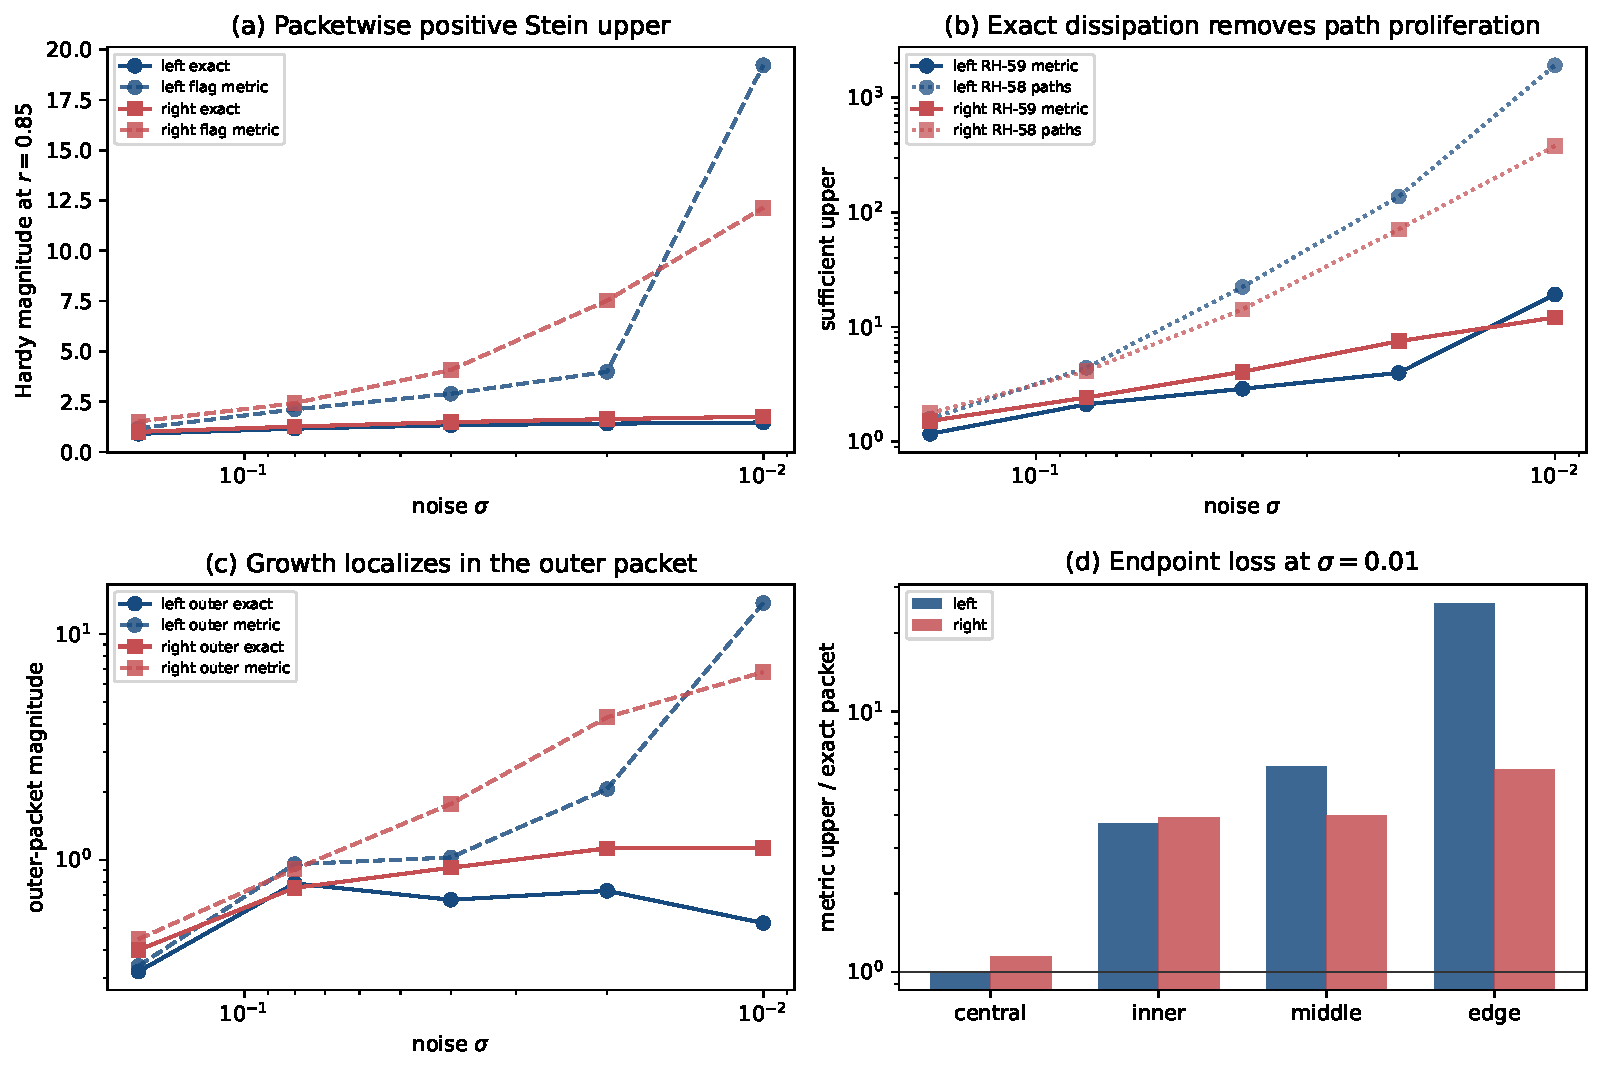
\includegraphics[width=\textwidth]{figures/flag_adapted_schur_stein.pdf}
\caption{Flag-metric audit.  (a) Packetwise positive Stein uppers versus the
exact energies.  (b) Exact dissipation removes most of the RH-58 path
proliferation.  (c) Remaining growth localizes in the outer packet.  (d) The
smallest-scale endpoint loss increases along the Schur flag.}
\label{fig:audit}
\end{figure}

\subsection{Outward-rounded model audit}

A 256-bit Arb calculation \citep{Johansson2017} evaluates
\eqref{eq:two-block} at
\[
 a=0.2,\quad b=0.7,\quad\gamma=0.3,\quad
 Y=(0.8,0.6),\quad(s_1,s_2)=(0.25,1).
\]
It encloses both local Lyapunov identities, proves $R\succ0$, inflates the
sharp multiplier by $1+10^{-6}$, verifies the resulting Stein supersolution
by strictly positive principal minors, and certifies the outer-packet upper.
This validates the formulas on the displayed scalar model only; no
production Schur metric is interval enclosed.

\section{Program consequence}
\label{sec:consequence}

\begin{description}[leftmargin=4.9cm,style=nextline]
 \item[Flag-metric existence]
 Closed for every stable finite Schur partition.  Diagonal-block
 compatibility is not the missing theorem.
 \item[Scalar absolute paths]
 Replaced.  Exact positive dissipation reduces the smallest-scale bounds by
 factors $100.0$ and $31.3$.
 \item[Central packet]
 Quantitatively mild; its local metric certificate is close to exact on the
 stored family.
 \item[Outer packet]
 Still obstructed.  Hierarchical scaling transfers the cost into the dual
 inner observation, and the fitted upper grows with a positive power.
 \item[Stage A1]
 Open.  Neither the metric absolute synthesis nor the empirical
 coherence-assisted variant supplies a polylogarithmic theorem.
 \item[Stage A4]
 Still conditional on Stage A1; the earlier factor and cutoff interfaces are
 unchanged.
\end{description}

The next target is therefore more specific than after RH-58.  A viable
argument must control the outer-to-inner observation channel without paying
for a nearly singular hierarchical metric.  Possibilities include a
frequency-localized observability inequality, a multiscale physical packet
basis whose outer injection is already aligned with the central channel, or
a phase-aware estimate for the off-diagonal packet Gram.  Reoptimizing the
same static block weights is unlikely to remove the endpoint tradeoff.

\section{No arithmetic or Hilbert--Polya conclusion}

Nothing here constructs a self-adjoint operator, a $T\log T$ counting law, a
von Mangoldt or prime-power trace formula, or a zeta-zero identity.  No
Riemann-hypothesis conclusion is drawn.  The independent twin-prime branch is
not used.

\section{Reproducibility}

The archive contains the flag-metric algebra, theorem tests, five-scale
all-column results, Arb model certificate, figures, dependency hashes, and
publication artifacts.  Principal commands are
\begin{verbatim}
PYTHONDONTWRITEBYTECODE=1 /root/math/.venv/bin/pytest -q -p no:cacheprovider
PYTHONDONTWRITEBYTECODE=1 /root/math/.venv/bin/python \
  experiments/run_flag_metric_pilot.py
PYTHONDONTWRITEBYTECODE=1 /root/math/.venv/bin/python \
  experiments/run_arb_flag_metric_audit.py
MPLBACKEND=Agg PYTHONDONTWRITEBYTECODE=1 /root/math/.venv/bin/python \
  experiments/make_figures.py
latexmk -pdf -interaction=nonstopmode -halt-on-error main.tex
\end{verbatim}

The flag-compatible metric, exact-dissipation supersolution, dominance
inequality, packet synthesis, and two-block tradeoff are analytic
finite-dimensional results.  All production asymptotics remain numerical.
Stage A1, unconditional intrinsic identification, and every arithmetic or
Hilbert--Polya conclusion remain outside the claims.

\bibliographystyle{plainnat}
\bibliography{references}
\end{document}
